%===============================================================================
% LaTeX sjabloon voor de bachelorproef toegepaste informatica aan HOGENT
% Meer info op https://github.com/HoGentTIN/latex-hogent-report
%===============================================================================
 
\documentclass[english,dit,thesis]{hogentreport}

\usepackage{lipsum} % For blind text, can be removed after adding actual content

%% Pictures to include in the text can be put in the graphics/ folder
\graphicspath{{graphics/}}

\usepackage[section,outputdir=../output]{minted}
\usepackage[section]{minted}
%% If you compile with the make_thesis.{bat,sh} script, use the following
%% import instead:
%% \usepackage[section,outputdir=../output]{minted}
\definecolor{bg}{RGB}{253,246,227} %% Set the background color of the codeframe

%% Change this line to edit the line numbering style:
\renewcommand{\theFancyVerbLine}{\ttfamily\scriptsize\arabic{FancyVerbLine}}

%% Macro definition to load external java source files with \javacode{filename}:
\newmintedfile[javacode]{java}{
    bgcolor=bg,
    fontfamily=tt,
    linenos=true,
    numberblanklines=true,
    numbersep=5pt,
    gobble=0,
    framesep=2mm,
    funcnamehighlighting=true,
    tabsize=4,
    obeytabs=false,
    breaklines=true,
    mathescape=false
    samepage=false,
    showspaces=false,
    showtabs =false,
    texcl=false,
}

% Other packages not already included can be imported here

%%---------- Document metadata -------------------------------------------------
\author{Jonathan Couck}
\supervisor{Mr. B. Vertonghen}
\cosupervisor{Mr. B. Vertonghen}
\title[Creation of a NuGet-package for faking authentication in a .Net application for faster development]%
{Fake authentication in .Net}
\academicyear{\advance\year by -1 \the\year--\advance\year by 1 \the\year}
\examperiod{2}
\degreesought{Bachelor of applied computer science}
\partialthesis{false} %% To display 'in partial fulfilment'
\institution{HOGENT}

%% Add global exceptions to the hyphenation here
\hyphenation{back-slash}

%% The bibliography (style and settings are  found in hogentthesis.cls)
\addbibresource{bachproef.bib}            %% Bibliography file
\addbibresource{../voorstel/voorstel.bib} %% Bibliography research proposal
\defbibheading{bibempty}{}

%% Prevent empty pages for right-handed chapter starts in twoside mode
\renewcommand{\cleardoublepage}{\clearpage}

\renewcommand{\arraystretch}{1.2}

%% Content starts here.
\begin{document}

%---------- Front matter -------------------------------------------------------

\frontmatter

\hypersetup{pageanchor=false} %% Disable page numbering references
%% Render a Dutch outer title page if the main language is English
\IfLanguageName{english}{%
    %% If necessary, information can be changed here
    \degreesought{Professionele Bachelor toegepaste informatica}%
    \begin{otherlanguage}{dutch}%
       \maketitle%
    \end{otherlanguage}%
}{}

%% Generates title page content
\maketitle
\hypersetup{pageanchor=true}

%%=============================================================================
%% Voorwoord
%%=============================================================================

\chapter*{\IfLanguageName{dutch}{Woord vooraf}{Preface}}%
\label{ch:voorwoord}

%% TODO:
%% Het voorwoord is het enige deel van de bachelorproef waar je vanuit je
%% eigen standpunt (``ik-vorm'') mag schrijven. Je kan hier bv. motiveren
%% waarom jij het onderwerp wil bespreken.
%% Vergeet ook niet te bedanken wie je geholpen/gesteund/... heeft

Before you lies the bachelors thesis `Fake authentication in Blazor: Creating a NuGet-package for faking authentication in a Blazor application for easier development`. This thesis is written to fulfil the graduation requirements of the  Applied Computer Science degree at HOGENT.

During the first semester of the school year '22-'23, I took the class 'Enterprise Web C\#' given by Mr. B. Vertonghen. In this class I was taught how to develop a complete application in the open-source web framework 'Blazor', developed by Microsoft. This also incorporated creating a fake authentication library which allowed for easy switching between regular users, admins, or users that aren't logged in.

During these classes Mr. Vertonghen also expressed his desire to simplify the process of authenticating a user, or at least temporarily doing so during the development stage of the app in question. This gave us the idea of creating a NuGet-package of the fake authentication for both front- and back-end.

I would like to thank my supervisor and cosupervisor, Mr. B. Vertonghen for the idea of this thesis and the guidance during the process of working on it. I learned a lot about creating a thesis, and also about myself.

I would also like to thank my family and friends for being there for me during tougher times.

I wish you much enjoyment in reading.

Jonathan Couck

Aalst, 13th of August 2023

\input{samenvatting}

%---------- Inhoud, lijst figuren, ... -----------------------------------------

\tableofcontents

% In a list of figures, the complete caption will be included. To prevent this,
% ALWAYS add a short description in the caption!
%
%  \caption[short description]{elaborate description}
%
% If you do, only the short description will be used in the list of figures

\listoffigures

% If you included tables and/or source code listings, uncomment the appropriate
% lines.
%\listoftables
%\listoflistings

% Als je een lijst van afkortingen of termen wil toevoegen, dan hoort die
% hier thuis. Gebruik bijvoorbeeld de ``glossaries'' package.
% https://www.overleaf.com/learn/latex/Glossaries

%---------- Kern ---------------------------------------------------------------

\mainmatter{}

% De eerste hoofdstukken van een bachelorproef zijn meestal een inleiding op
% het onderwerp, literatuurstudie en verantwoording methodologie.
% Aarzel niet om een meer beschrijvende titel aan deze hoofdstukken te geven of
% om bijvoorbeeld de inleiding en/of stand van zaken over meerdere hoofdstukken
% te verspreiden!

%%=============================================================================
%% Inleiding
%%=============================================================================

\chapter{\IfLanguageName{dutch}{Inleiding}{Introduction}}%
\label{ch:inleiding}

Arguably the most important factor of a modern applications is its safety. Part of ensuring that is making sure the users are authenticated in a proper way. These applications increasingly use different types of ways to authenticate a user. The most commonly used methods are listed by \textcite{Hassan2017}: Session based, token based, passwordless, single sign on, social sign-in and two-factor authentication. In another article, \textcite{Maayan} concludes: `Authentication technology is always changing. Businesses have to move beyond passwords and think of authentication as a means of enhancing user experience. As a result of enhanced authentication methods and technologies, attackers will not be able to exploit passwords, and a data breach will be prevented`.

For the developer, this means keeping track of the latest technologies and how to implement them into new projects. This fact makes it very difficult to choose a fitting authentication technology right at the beginning stages of development. In other cases it might be that for example higher ups from corporate want a simple version at first, so that test users can ultimately decide what technology should be used in the final product. Of course in these cases it is not an option to wait around for those results and waste time by contemplating about this decision.

Imagine a scenario. The development of a new high-tech webshop app is halfway done. In the beginning the developers decided on two-factor authentication as the way to go for this specific project. At this time they are busy debugging a certain issue with the shopping cart. They want to test the newly written code, so they log in as a regular user first, put a product in the shopping cart, log back out again, log back in as an admin, change some information of the product, and then log back in as a regular user to see if the app is performing as it is supposed to. This appears to be a frustrating process that should be able to be done quicker.

All of these cases are examples of where a fake authentication service could help progress by quite a bit. If developed correctly, this service could switch the type of user with just the click of one button, instead of having to go through the entire login process.

\section{\IfLanguageName{dutch}{Probleemstelling}{Problem Statement}}%
\label{sec:probleemstelling}

As mentioned before, not having a straight answer to what type of authentication will be used in an app or using one that will take up time in the development process can ben a time costly procedure. This of course is something companies want to avoid. It can partly be resolved by planning ahead of time, and going over the possible options before starting development. Unfortunately though plans do sometimes change, and to then throw a big part of the authentication overboard is not ideal.

The advantages and disadvantages of early and late implementation of the authentication service are looked at from the standpoint of the developer.

\section{\IfLanguageName{dutch}{Onderzoeksvraag}{Research question}}%
\label{sec:onderzoeksvraag}

%TODO

Wees zo concreet mogelijk bij het formuleren van je onderzoeksvraag. Een onderzoeksvraag is trouwens iets waar nog niemand op dit moment een antwoord heeft (voor zover je kan nagaan). Het opzoeken van bestaande informatie (bv. ``welke tools bestaan er voor deze toepassing?'') is dus geen onderzoeksvraag. Je kan de onderzoeksvraag verder specifiëren in deelvragen. Bv.~als je onderzoek gaat over performantiemetingen, dan 

\section{\IfLanguageName{dutch}{Onderzoeksdoelstelling}{Research objective}}%
\label{sec:onderzoeksdoelstelling}

The objective of this thesis is to have two working prototype NuGet-packages, one for client-side, one for server-side, that can be downloaded and applied to any ASP.NET-application. These packages should be able to provide the following:

\begin{itemize}
    \item switching between authentication methods
    \item adding as many personalized types of users as needed
    \item identify if a user is logged in
    \item registering a new user
    \item logging in as a user
    \item personalize information stored of user
\end{itemize}

\section{\IfLanguageName{dutch}{Opzet van deze bachelorproef}{Structure of this bachelor thesis}}%
\label{sec:opzet-bachelorproef}


% Het is gebruikelijk aan het einde van de inleiding een overzicht te
% geven van de opbouw van de rest van de tekst. Deze sectie bevat al een aanzet
% die je kan aanvullen/aanpassen in functie van je eigen tekst.

De rest van deze bachelorproef is als volgt opgebouwd:

In Hoofdstuk~\ref{ch:stand-van-zaken} wordt een overzicht gegeven van de stand van zaken binnen het onderzoeksdomein, op basis van een literatuurstudie.

In Hoofdstuk~\ref{ch:methodologie} wordt de methodologie toegelicht en worden de gebruikte onderzoekstechnieken besproken om een antwoord te kunnen formuleren op de onderzoeksvragen.

% TODO: Vul hier aan voor je eigen hoofstukken, één of twee zinnen per hoofdstuk

In Hoofdstuk~\ref{ch:conclusie}, tenslotte, wordt de conclusie gegeven en een antwoord geformuleerd op de onderzoeksvragen. Daarbij wordt ook een aanzet gegeven voor toekomstig onderzoek binnen dit domein.
\chapter{\IfLanguageName{dutch}{Stand van zaken}{State of the art}}%
\label{ch:stand-van-zaken}

% Tip: Begin elk hoofdstuk met een paragraaf inleiding die beschrijft hoe
% dit hoofdstuk past binnen het geheel van de bachelorproef. Geef in het
% bijzonder aan wat de link is met het vorige en volgende hoofdstuk.

% Pas na deze inleidende paragraaf komt de eerste sectiehoofding.

In this chapter the research domain of authentication is mapped out by answering a few questions that will help decide certain factors that are important for creating the fake authentication packages. Among these factors are:

\begin{itemize}
    \item the method of authenticating
    \item user role customization (+ mock data generation) %TODO weghalen
    \item security best practices
    \item creating and publishing a NuGet package
\end{itemize}

\section{State of authentication}

To discuss the factors needed to create the packages, the current state of authentication needs to be explored first.

\subsection{AAA}

When talking about authentication one often hears about triple-A. When these are mentioned they refer to: 

\begin{itemize}
    \item authentication
    \item authorization
    \item accounting
\end{itemize}

\subsubsection{Authentication}

\textcite{Magnusson2022} describes authentication as the process of identifying a user and granting them access to the network. The server evaluates the credential data submitted by the user compared to the ones stored in the network's database.

\subsubsection{Authorization}

Authorization on the other hand enforces the network policies, granular access control and user privileges. The cybersecurity AAA protocol determines which specific network resources the user has permission to access, such as a particular application, database or online service.

\subsubsection{Accounting}

Lastly, accounting is all about measuring what is happening within the network. This could mean collecting and logging data on user sessions, such as length of time, type of session, resource usage. The value here is that it offers a clear audit trail for compliance and business purposes.

\subsection{Different authentication methods}
\label{ch:different-authentication-methods}

In this day and age we have a lot more ways of authenticating a user than just writing a username or email address secured with a single password. \textcite{Maayan} lists the five most popular ways in his article and explains them.

\subsubsection{Password-based authentication}

Passwords are the most common methods of authentication. Passwords can be in the form of a string of letters, numbers, or special characters. To protect yourself you need to create strong passwords that include a combination of all possible options. 

However, passwords are prone to phishing attacks and bad hygiene that weakens effectiveness. An average person has about 25 different online accounts, but only 54\% of users use different passwords across their accounts. 

The truth is that there are a lot of passwords to remember. As a result, many people choose convenience over security. Most people use simple passwords instead of creating reliable passwords because they are easier to remember. 

The bottom line is that passwords have a lot of weaknesses and are not sufficient in protecting online information. Hackers can easily guess user credentials by running through all possible combinations until they find a match.

An article on \textcite{Descope2023} states both the pros and cons of this method. The pros being familiarity, affordability and user control, while the cons are its vulnerability, predictability, fallibility and complexity.

\subsubsection{Multi-factor authentication}

Multi-Factor Authentication (MFA) is an authentication method that requires two or more independent ways to identify a user. Examples include codes generated from the user’s smartphone, Captcha tests, fingerprints, voice biometrics or facial recognition. 

MFA authentication methods and technologies increase the confidence of users by adding multiple layers of security. MFA may be a good defence against most account hacks, but it has its own pitfalls. People may lose their phones or SIM cards and not be able to generate an authentication code.

An article on \textcite{Mitek2021} states both the benefits and costs of multi-factor authentication. The benefits are and improved user experience, greater security, protection against brute force attacks and reduced cost in the long run. The costs on the other hand are consumer friction, bias and inaccuracy, and a high implementation cost.

\subsubsection{Certificate-based authentication}

Certificate-based authentication technologies identify users, machines or devices by using digital certificates. A digital certificate is an electronic document based on the idea of a driver’s license or a passport. 

The certificate contains the digital identity of a user including a public key, and the digital signature of a certification authority. Digital certificates prove the ownership of a public key and issued only by a certification authority. 

Users provide their digital certificates when they sign in to a server. The server verifies the credibility of the digital signature and the certificate authority. The server then uses cryptography to confirm that the user has a correct private key associated with the certificate.

When looking for the advantages of certificate-based authentication, \textcite{Spector} says: `The biggest advantages of digital certificate-based authentication are privacy-based. By encrypting your communications — emails, logins or online banking transactions — digital certificates protect your private data and prevent the information from being seen by unintended eyes. Digital certificate systems are also user-friendly, usually working automatically and requiring minimal action or involvement from either senders or recipients. Microsoft states that certificate servers are cheaper and easier to manage than other certificate authorities or systems used for encryption.`

When talking about the disadvantages he says: `While the idea of digital certificates is to block outsiders from intercepting your messages, the system is not an infallible one. In 2011, for example, a Dutch digital certificate authority called DigiNotar was compromised by hackers. Since certificate authorities are the ones in charge of issuing digital certificates (think of them as the digital version of a passport office), hackers often target these authorities in order to manipulate certificate information. As a result, when a certificate authority is compromised, hackers can create websites or send emails that look genuine and pass certification tests, but are actually fraudulent.`

\subsubsection{Biometric authentication}

Biometrics authentication is a security process that relies on the unique biological characteristics of an individual. Here are key advantages of using biometric authentication technologies.

Biometric authentication technologies are used by consumers, governments and private corporations including airports, military bases, and national borders. The technology is increasingly adopted due to the ability to achieve a high level of security without creating friction for the user. Common biometric authentication methods include facial and speaker recognition and fingerprint scanners.

For the advantages \textcite{Perez2022} lists enhanced security, convenience and an improved user experience. The disadvantages that face this method are privacy concerns, false positives and again a high cost.

\subsubsection{Token-based authentication}

Token-based authentication technologies enable users to enter their credentials once and receive a unique encrypted string of random characters in exchange. You can then use the token to access protected systems instead of entering your credentials all over again. The digital token proves that you already have access permission. Use cases of token-based authentication include RESTful APIs that are used by multiple frameworks and clients.

For this implementation \textcite{Malviya} gives the major pros and cons. The pros are its scalability, efficiency, flexibility, performance and robust security. The cons are a possibility of a compromised secret key, data overhead and a shorter lifespan.

\subsection{Token-based authentication}

An article in \textcite{Okta2023}, a pioneering company in authentication that created OAuth, Okta SSO and more widely acclaimed products, lists the three different types of authentication tokens.

\begin{itemize}
    \item Connected: Keys, discs, drives, and other physical items plug into the system for access. If you've ever used a USB device or smartcard to log into a system, you've used a connected token.
    \item Contactless: A device is close enough to a server to communicate with it, but it doesn't plug in. Microsoft's so-called "magic ring" would be an example of this type of token.
    \item Disconnected: A device can communicate with the server across long distances, even if it never touches another device at all. If you've ever used your phone for a two-factor authentication process, you've used this type of token.
\end{itemize}

When thinking of the fake authentication service, it is apparent that the third option, disconnected tokens, will be the ones used in the packages.

The article also shows the four steps in the process of token authentication. First is the request. The person asks for access to a server or protected resource. That could involve a login with a password, or it could involve some other process you specify. Then comes the verification. The server determines that the person should have access. That could involve checking the password against the username, or it could involve another process you specify. After verification, the server issues a token and passes it to the user. Lastly comes storage, meaning that the token sits within the user's browser while work continues.

\subsection{Which type of method will be implemented}

When comparing the pros and cons of the methods mentioned in chapter~\ref{ch:different-authentication-methods}, token-based authentication immediately jumps out as the top candidates to implement in the fake authentication packages. With its great scalability, efficiency, flexibility and performance being very important factors for this use case. Since these packages is only meant to be used during the development stages, it is also worth mentioning that the cons are things that will not matter here. The compromised secret key can be changed during development, the shorter lifespan can be lengthened for a while and since there isn't actual data being sent to a remote server for example, the data overhead shouldn't matter that much either. All in all, this seems like the perfect candidate.

\subsection{Encoding vs Encrypting}

When certain data is transported from server to client it is often either encoded or encrypted. These are terms commonly interchanged. Both are used to transform data into a different format, but they have certain differences that are be explained by \textcite{CoderSaty}.

\subsubsection{Encrypting}

Encrypting is a process used to convert simple readable data known as plain text to unreadable data known as ciphertext which can only be converted to plain text if the user knows the encryption key. It is used basically to keep our data safe. The main purpose of the encryption is to convert our data in such a form that it is garbage for the person who does not know the encryption key. It is used to prevent unauthorized access. The reverse of encryption is decryption and it is used to get back the plain text from the ciphertext. For decryption, we must know the encryption key and the encryption algorithm \autocite{CoderSaty}. 

The encrypted data is just treated like other data. We can also use more than one encryption algorithm on the same data. The real-life examples are sending someone a secret message that only they should be able to read, or securely sending a password over the Internet. The goal is data confidentiality.

\subsubsection{Encoding}

It is the process to transform data in such a format that it can be easily used by different types of systems. The algorithm used to encode the data is publicly available and it can be easily decoded in the readable form if the person knows the algorithm. It does not require any key to decode the information. The main purpose is data usability instead of confidentiality. The main aim of encoding is to transform the data so that it can be properly used by a different type of system. It is not used to protect the data as it is easy to reverse in comparison to encryption \autocite{CoderSaty}.

Encoding is the way to go for this project since it is a developer tool, and doesn't have the need for preventing unauthorized access to the data within the token.

\subsection {Token encoding}
\label{ch:token-encoding}

Choosing an encoding method for a token involves considering various factors, like compatibility, readability, space efficiency. The most common ways used to encode a token are Uniform Resource Locator (URL), Base64, American Standard Code for Information Interchange (ASCII) and Json Web Token (JWT) encoding.

\subsubsection{URL}

URL encoding, officially known as percent-encoding, is a method to encode arbitrary data in a Uniform Resource Identifier (URI) using only the limited US-ASCII characters legal within a URI \autocite{Wikipedia2023}.

\subsubsection{Base64}

Base64 is a group of similar binary-to-text encoding schemes that represent binary data in an ASCII string format by translating it into a radix-64 representation. The term Base64 originates from a specific MIME content transfer encoding \autocite{Mozilla2023}.

When the term "Base64" is used on its own to refer to a specific algorithm, it typically refers to the version of Base64 outlined in RFC 4648, section 4, which uses the following alphabet to represent the radix-64 digits, alongside = as a padding character: ABCDEFGHIJKLMNOPQRSTUVWXYZabcdefghijklmnopqrstuvwxyz0123456789+/

\subsubsection{ASCII}

ASCII is a character encoding standard for electronic communication. ASCII codes represent text in computers, telecommunications equipment, and other devices. Because of technical limitations of computer systems at the time it was invented, ASCII has just 128 code points, of which only 95 are printable characters, which severely limited its scope. Many computer systems instead use Unicode, which has millions of code points, but the first 128 of these are the same as the ASCII set \autocite{Wikipedia2023a}.

\subsubsection{JWT}

JWT is an open standard that defines a compact and self-contained way for securely transmitting information between parties as a JSON object. This information can be verified and trusted because it is digitally signed. JWTs can be signed using a secret (with the HMAC algorithm) or a public/private key pair using RSA or ECDSA \autocite{JWT}.

In its compact form, JSON Web Tokens consist of three parts separated by dots (.), which are the header, payload and signature. Therefore, a JWT typically looks like the following: xxxxx.yyyyy.zzzzz

The header typically consists of two parts: the type of the token, which is JWT, and the signing algorithm being used, such as HMAC SHA256 or RSA. Then, this JSON is Base64Url encoded to form the first part of the JWT.

The second part of the token is the payload, which contains the claims. Claims are statements about an entity (typically, the user) and additional data. The payload is then Base64Url encoded to form the second part of the JSON Web Token.

To create the signature part you have to take the encoded header, the encoded payload, a secret, the algorithm specified in the header, and sign that.

\subsubsection{Implementing}

The goal of these packages would be to make any of these possible to implement and use, however starting out only two of these will be implemented. These packages however will be with the thought in mind that this should be as easy as possible to expand and add extra encoding methods.

As per request of Mr. Vertonghen, JWT should definitely be one of the methods implemented. Besides JWT Base64 will also be implemented, since this is one of the more basic methods of encoding binary data and it is used often in simple HTTP authentication to encode the credentials \autocite{JavaTPoint}.

\subsection{Authorization patterns}

In authorization, there are different ways a user can be given permissions. This part of the thesis goes through five of the most common ones.

\begin{itemize}
    \item Roles as User Properties
    \item Group-Based Roll-Based Access Control (RBAC)
    \item Group-Based RBAC with Fine-Grained Permissions
    \item Fine-Grained Authorization for Domain-Specific Objects
    \item Combining Group-Based RBAC and FGA
\end{itemize}

\subsubsection{Roles as User Properties}

The simplest authorization pattern models a set of roles as properties of the user. These roles can be configured in the identity provider (IDP) and are often embedded as scopes in the access token generated by the IDP \autocite{Gazitt2023}.

\subsubsection{Group-Based RBAC}

The next pattern relies on groups (and group hierarchies) as a way to organize users.

Most applications have coarse-grained roles, such as “super-admin,” “admin,”  “editor,” “viewer,” “billing-admin,” that determine permissions to objects across the entire tenant.

These roles are typically assigned by making a user a member of a group. The group membership means that the user has been granted a role. Groups can be organized into hierarchies. For example, the “auditor” group can include “internal-auditors” and “external-auditors.” These two groups can in turn include specific users \autocite{Gazitt2023}.

\subsubsection{Group-Based RBAC with Fine-Grained Permissions}

A more scalable authorization system will define a set of discrete permissions and assign those to roles. Authorization systems often define permissions as first-class concepts. Instead of checking whether a user is a member of a group, the policy can check whether a user has permission.

\subsubsection{Fine-Grained Authorization (FGA) for Domain-Specific Objects}

So far we’ve been dealing with “global” roles. Many applications want to grant permissions on a set of objects that they manage. For example, a file-sharing application such as Google Drive defines “folders” and “files” as object types. Folders and files can both have a parent folder. Each of these objects has a set of relations (“owner,” “editor,” “commenter” and “viewer”) and the “owner” can grant these roles to users and groups. So rather than a global “editor” role which has edit access to every file and folder, these permissions can be assigned to discrete folders and files.

\subsubsection{Combining Group-Based RBAC and FGA}

Most real-world applications implement some combination of group-based RBAC and fine-grained authorization. Often, authorization includes checking a global role (e.g., “editor”) and then checking whether the user has access to a particular resource (e.g., a list). The user needs to satisfy both conditions to be able to edit items on that list.

\section{NuGet package}

An essential tool for any modern development platform is a mechanism through which developers can create, share, and consume useful code. Often such code is bundled into "packages" that contain compiled code (as DLLs) along with other content needed in the projects that consume these packages. For .NET (including .NET Core), the Microsoft-supported mechanism for sharing code is NuGet, which defines how packages for .NET are created, hosted, and consumed, and provides the tools for each of those roles \autocite{Microsoft2022}.

\subsection{What is a NuGet package}

Put simply, a NuGet package is a single ZIP file with the .nupkg extension that contains compiled code (DLLs), other files related to that code, and a descriptive manifest that includes information like the package's version number. Developers with code to share create packages and publish them to a public or private host. Package consumers obtain those packages from suitable hosts, add them to their projects, and then call a package's functionality in their project code. NuGet itself then handles all of the intermediate details \autocite{Microsoft2022}.

Because NuGet supports private hosts alongside the public nuget.org host, you can use NuGet packages to share code that's exclusive to an organization or a work group. You can also use NuGet packages as a convenient way to factor your own code for use in nothing but your own projects. In short, a NuGet package is a shareable unit of code, but does not require nor imply any particular means of sharing \autocite{Microsoft2022}.

\begin{figure}
    \centering
    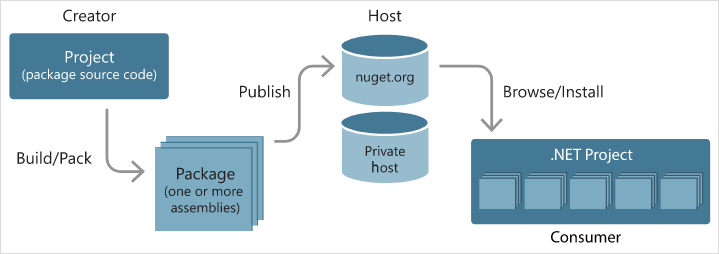
\includegraphics[scale=0.75]{nuget-flow.png}
    \caption{The flow of packages}
    \label{fig:nuget-flow}
\end{figure}

\subsection{Creating a NuGet package}

In the \textcite{Microsoft2022a} guide for package creation, it is stated that creating a package starts with the compiled code (typically .NET assemblies) that you want to package and share with others, either through the public nuget.org gallery or a private gallery within your organization. The package can also include additional files such as a readme that is displayed when the package is installed, and can include transformations to certain project files.

Creating a package is possible with the dotnet CLI, the nuget.exe CLI or MSBuild. In this case the dotnet CLI will be used.

The \textcite{Microsoft2022b} article explains all steps for creating a NuGet package using the dotnet CLI.

\subsubsection{Set properties}

You can create an example class library project by using the dotnet new classlib command, and package the project by using dotnet pack. The dotnet pack command uses the following properties.

\begin{itemize}
    \item PackageId is the package identifier and must be unique across nuget.org
    \item Version is a specific version number in the form Major.Minor.Patch[-Suffix]
    \item Authors are the authors of the package
    \item Company is company information
    \item Product is product information
\end{itemize}

If you don't specify values in the project file, the command uses default values. In Visual Studio these values can be set in the project properties.

\begin{verbatim}
    <Project Sdk="Microsoft.NET.Sdk">
        <PropertyGroup>
            <TargetFramework>netstandard2.0</TargetFramework>
            <PackageId>UniqueID</PackageId>
            <Version>1.0.0</Version>
            <Authors>Author Name</Authors>
            <Company>Company Name</Company>
            <Product>Product Name</Product>
        </PropertyGroup>
    </Project>
\end{verbatim}

The package's optional description appears on the README tab of the package's nuget.org page. The description pulls from the <Description> in the project file.

\subsubsection{Run the pack command}

To build the NuGet package or .nupkg file, run the dotnet pack command from the project folder, which also builds the project automatically. After this, the package can be published to the host of your choice.

\subsection{Publishing a NuGet package}

As stated before, NuGet packages can either be published publicly or privately. In this case, the package will be published publicly.

After creating an account on nuget.org, the next steps are needed to have a package uploaded \autocite{Microsoft2022c}:

\begin{itemize}
    \item Select Upload on the top menu at nuget.org, browse to the package on your computer, and select Open. If the package ID already exists on nuget.org, you get an error. Change the package identifier in your project, repack, and try the upload again.
    \item If the package name is available, the Verify section opens so you can review the metadata from the package manifest. If you included a readme file in your package, select Preview to make sure all content renders properly.
    \item When all the information is ready, select Submit.
\end{itemize}




%%=============================================================================
%% Methodologie
%%=============================================================================

\chapter{\IfLanguageName{dutch}{Methodologie}{Methodology}}%
\label{ch:methodologie}

Like any thesis, this one starts with a comprehensive literature study of the research domain and of the technologies used. The goal of this chapter is to get a clear answer to which of the different routes these packages could go on should be chosen. This literature study can be found in chapter~\ref{ch:stand-van-zaken}

After the literature study, the fake authentication packages will be created. The creation of these packages can be found in chapter~\ref{ch:fake-auth}. The first section explains the initial state of the application created by Mr. Vertonghen. The flow of data in the new fake authentication is further expanded upon. The design decisions are described and all the ways modular programming is used for separating classes and methods into independent pieces are shown.

The code is now written, and needs to be turned into the two packages and set free to the public so that it can be used in future projects. The creation publishing process of these packages is detailed and whether or not there were any problems encountered during this process.

Lastly a detailed way of how to install, implement and customize the packages is written down and eventually a medium.com article could be published, depending on whether or not this can be done in time. If this article is not able to be created, this explanation will of course still be available in the README of the packages.


% Voeg hier je eigen hoofdstukken toe die de ``corpus'' van je bachelorproef
% vormen. De structuur en titels hangen af van je eigen onderzoek. Je kan bv.
% elke fase in je onderzoek in een apart hoofdstuk bespreken.

\chapter{Fake authentication creation}
\label{ch:fake-auth2}

After all this research, it is finally time to start coding the fake authentication packages. In this chapter the application that the packages was initially made around and tested for is clarified. This simple webshop was created for the course Enterprise Web C\#, given by Mr. Vertonghen to students at Hogeschool Gent. After this, the flow of data in the packages is described. Then the three different projects created are looked at in detail, to find out the magic behind the packages.

\section{Initial application}

As said before, the initial application that was used to create the packages is a simple webshop called The Bogus Store. It was created by Mr. Vertonghen for the course Enterprise Web C\# at Hogeschool Gent to teach students how to create applications in .Net. The repository can be found at \href{https://github.com/HOGENT-Web/csharp-ch-8-example-2}{this repository}. The reason this specific version of the application was used, is that it had a couple of nice looking pages on the client side, but also had a fake authentication that is used. The solution-branch was used since this had a couple extra features handy for testing the new fake authentication.

The application itself is a webshop, where users can view a list products, view the details of these products and then decide to put these in a shopping cart and order them. The functionality of ordering isn't implemented. There are different roles or personas available for choosing. These roles are displayed in a list, and thanks to a fake authentication that is already in place, these can be switched between very easily. When choosing the Administrator persona, it is apparent that two more tabs open up in the menu, Tags and Customers. These two routes are protected and only the Administrator, who of course has a role of the same name, can access these routes. This means that when these routes are accessed by anyone else, a `Not authorized` message pops up.

\subsection{Fake authentication}

In this application, a fake authentication is already in place. Let's run through how this works exactly.

\subsubsection{Client}

When starting up a client a singleton FakeAuthenticationProvider is set in the Program.cs file. This means only a single instance of itself is created, which can then be injected into other classes, so that whenever a FakeAuthenticationProvider object has to be used, it comes back to that particular instance. This FakeAuthenticationProvider is a derived class of AuthenticationStateProvider, which is a class of the Microsoft.AspNetCore.Components.Authorization package that provides information about the authentication state of a user.

\begin{verbatim}
    builder.Services.AddSingleton<FakeAuthenticationProvider>();
    builder.Services.AddScoped<AuthenticationStateProvider>(provider => provider.GetRequiredService<FakeAuthenticationProvider>());
    builder.Services.AddTransient<FakeAuthorizationMessageHandler>();
    
    builder.Services.AddHttpClient("Project.ServerAPI", client => client.BaseAddress = new Uri(builder.HostEnvironment.BaseAddress))
    .AddHttpMessageHandler<FakeAuthorizationMessageHandler>();
\end{verbatim}

This class looks like the following:

\begin{verbatim}
    public class FakeAuthenticationProvider : AuthenticationStateProvider
    {
        public static ClaimsPrincipal Anonymous => new(new ClaimsIdentity(new[]
        {
            new Claim(ClaimTypes.Name, "Anonymous"),
        }));
        
        public static ClaimsPrincipal Administrator => new(new ClaimsIdentity(new[]
        {
            new Claim(ClaimTypes.NameIdentifier, "1"),
            new Claim(ClaimTypes.Name, "Administrator"),
            new Claim(ClaimTypes.Email, "fake-administrator@gmail.com"),
            new Claim(ClaimTypes.Role, Roles.Administrator),
        }, "Fake Authentication"));
        
        public static ClaimsPrincipal Customer => new(new ClaimsIdentity(new[]
        {
            new Claim(ClaimTypes.NameIdentifier, "2"),
            new Claim(ClaimTypes.Name, "Customer"),
            new Claim(ClaimTypes.Email, "fake-customer@gmail.com"),
            new Claim(ClaimTypes.Role, Roles.Customer),
        }, "Fake Authentication"));
        
        public static IEnumerable<ClaimsPrincipal> ClaimsPrincipals =>
            new List<ClaimsPrincipal>() { Anonymous, Customer, Administrator }; 
        
        public ClaimsPrincipal Current { get; private set; } = Administrator;
        
        public override Task<AuthenticationState> GetAuthenticationStateAsync()
        {
            return Task.FromResult(new AuthenticationState(Current));
        }
        
        public void ChangeAuthenticationState(ClaimsPrincipal claimsPrincipal)
        {
            Current = claimsPrincipal;
            NotifyAuthenticationStateChanged(GetAuthenticationStateAsync());
        }
    }
\end{verbatim}

In this class three ClaimsPrincipals are made, each with its own ClaimsIdentity, and with that ClaimsIdentity the Claims that belong to that particular persona. These ClaimsPrincipal objects are then gathered in a List. Also a Current ClaimsPrincipal is set, that holds the currently logged in persona. Remember that this class is made as a singleton, so all of this information is then made available to the entire application by injection. This class also has two methods. GetAuthenticationStateAsync, which is overridden from AuthenticationStateProvider and returns a new AuthenticationState with the current logged in persona and its Claims. The second method is ChangeAuthenticationState which sets the current persona to a new one and notifies the application that the authentication state has changed.

After the creation of the HttpClient, a FakeAuthorizationMessageHandler is attached to it. This message handler intercepts any request sent by the client, and adds the appropriate Headers to it if the current user is not the anonymous one.

\begin{verbatim}
    public class FakeAuthorizationMessageHandler : DelegatingHandler
    {
        private readonly FakeAuthenticationProvider fakeAuthenticationProvider;
        
        public FakeAuthorizationMessageHandler(FakeAuthenticationProvider fakeAuthenticationProvider)
        {
            this.fakeAuthenticationProvider = fakeAuthenticationProvider;
        }
        protected override Task<HttpResponseMessage> SendAsync(HttpRequestMessage request, System.Threading.CancellationToken cancellationToken)
        {
            if(fakeAuthenticationProvider.Current.Identity?.Name == FakeAuthenticationProvider.Anonymous.Identity?.Name)
            {
                return base.SendAsync(request, cancellationToken);
            }
            
            request.Headers.Add("UserId", fakeAuthenticationProvider.Current.FindFirst(ClaimTypes.NameIdentifier)?.Value);
            request.Headers.Add("Role", fakeAuthenticationProvider.Current.FindFirst(ClaimTypes.Role)?.Value);
            request.Headers.Add("Email", fakeAuthenticationProvider.Current.FindFirst(ClaimTypes.Email)?.Value);
            request.Headers.Add("Name", fakeAuthenticationProvider.Current.FindFirst(ClaimTypes.Name)?.Value);
            return base.SendAsync(request, cancellationToken);
        }
    }
\end{verbatim}

At this time the current persona can be changed by calling the ChangeAuthenticationState method of the FakeAuthenticationProvider, and this is done in the AccessControl razor component. When this method is called, the menu on top changes, because of an AuthorizeView, which checks the current user for the correct role. The same can be done with a specific route by adding \texttt{@attribute [Authorize(Roles = Roles.Administrator)]} to the top of the razor file.

\subsubsection{Server}

In the Program.cs file authentication is added to the services by the following line of code:

\begin{verbatim}
    
    builder.Services.AddAuthentication("Fake Authentication")
        .AddScheme<AuthenticationSchemeOptions, FakeAuthenticationHandler>("Fake Authentication", null);
\end{verbatim}

A new FakeAuthenticationHandler object is set as the handler for this service. This FakeAuthenticationHandler is derived from the AuthenticationHandler class, which comes from the Microsoft.AspNetCore.Authentication package. This class overrides a single method called HandleAuthenticateAsync.

\begin{verbatim}
    
    protected override async Task<AuthenticateResult> HandleAuthenticateAsync()
    {
        List<Claim> claims = new();
        
        if (Context.Request.Headers.TryGetValue("UserId", out var userId))
        {
            claims.Add(new Claim(ClaimTypes.NameIdentifier, userId!));
        }
        
        if (Context.Request.Headers.TryGetValue("Role", out var roles))
        {
            claims.Add(new Claim(ClaimTypes.Role, roles!));
        }
        
        if (Context.Request.Headers.TryGetValue("Email", out var email))
        {
            claims.Add(new Claim(ClaimTypes.Email, email!));
        }
        
        if (Context.Request.Headers.TryGetValue("Name", out var name))
        {
            claims.Add(new Claim(ClaimTypes.Name, name!));
        }
        
        if (claims.Any())
        {
            var identity = new ClaimsIdentity(claims, Scheme.Name);
            var principal = new ClaimsPrincipal(identity);
            var ticket = new AuthenticationTicket(principal, Scheme.Name);
            return await Task.FromResult(AuthenticateResult.Success(ticket));
        }
        
        return await Task.FromResult(AuthenticateResult.NoResult());
        
    }
\end{verbatim}

What this method does is, whenever a request comes in to the server, it searches the headers for four values (UserId, Role, Email and Name). These are the four values that were set by the client whenever a request was sent out with a current user that is not anonymous. If they are found these claims are then added to a ClaimsIdentity in a new ClaimsPrincipal. Lastly a AuthenticateResult is then returned from this ClaimsPrincipal.

All that is left to do when checking whether or not a request is made by a valid user, is to add either \texttt{[HttpGet, AllowAnonymous]} or \texttt{[HttpPost, Authorize(Roles = Roles.Administrator)]} to a method in the controllers. This returns a 401 Error if the user is not authorized.

\section{Flow of data}

After understanding the initial situation, let's take a look at how this changed when adding the new fake authentication.

Here, minimal information about the methods is given. Any code written is be looked at further in detail in the sections \ref{ch:package-server}, \ref{ch:package-client} and \ref{ch:package-shared}.

When looking at the flow of data in the application now, it makes more sense to start with the server.

One more thing that needs to be made clear, when talking about the 'Server' or the 'Client', the server and client of the application are meant. When talking the 'FakeAuth.Server' or the 'FakeAuth.Client', the packages of the fake authentication are meant.

\subsection{Server}

When starting the application, the first file that is run through is the Program.cs of the Server.

\subsubsection{Program.cs}

The first thought that occurs is that this package should only ever be used in development, never on production or staging. Knowing this, the if-statement that checks whether or not the app is running in development can comfortably be added. When implementing the actual authentication system, an else can be used to configure this on production or staging.

Next, a singleton is added to the builder of type ITokenGeneratorService. This singleton can for now contain either a JwtTokenGeneratorService or a BasicTokenGeneratorService, but this is easily expanded upon to other token types. Both of these are derived from the ITokenGeneratorService interface. This interface implements a method called GenerateToken, that requires a FakeIdentity object and generates an object of type Token.

\subsubsection{FakeIdentity}

The FakeIdentity class is a class that is created to contain all information around a certain persona or role, depending on how the user wants to use the packages.

This FakeIdentity contains a name, role and claims. The name and role are both set to `Anonymous` if they are not given in the creation. It has a method that checks if it is anonymous, and a method that returns a FakeIdentityDto.Index to use for data transfer. The last method turns this FakeIdentity into an object of type ClaimsIdentity, adding both its name and role to the claims.

\subsubsection{Token}

The Token class is a simple class that contains the token string, duration of the token, the FakeIdentity it was issued for and the type of token (for now JWT or Base64).

\subsubsection{ITokenGeneratorService}

Now let's circle back to the ITokenGeneratorService interface. This is the service that generates the token when given all information through a FakeIdentity object. Later a deeper look is given into how this exactly works

\subsubsection{FakeAuthServerExtensions}

The next step is to add the fake authentication to the Server. This is done with the FakeAuthServerExtensions static class. It only has one static method which is used in the Program.cs file of the Server. It requires two types, one derived from ITokenGeneratorService, and one from AuthenticationHandler. These should be representative of which method of encoding is chosen. For example with JWT, this would JwtTokenGeneratorService and JwtAuthenticationHandler.

The AddFakeAuthentication method is used to connect the Server with the FakeAuth.Server package. This method fetches the configuration from the appsettings file of the Server, sets the FakeIdentityService needed for saving the identities and exchanging these between the Server and Client. From the configuration the JWT settings are captured and entered into a JwtConfig object if needed. This object holds the audience, issuer, key and duration needed for creating a JWT token.

\subsubsection{FakeIdentityService}

This class is used as a singleton, set in the AddFakeAuthentication method. It is used to store the identities set in the appsettings of the Server. Also in this service included is a method for finding the identity linked with a certain name. Lastly on creation a method is called which checks the given identities for an anonymous one. If it is not present, one is created, since an anonymous identity is necessary for the app to work, and it is a given that every application should have an anonymous identity, even if it doesn't have any rights to pages or routes.

\subsubsection{FakeAuthController}

The last part of the flow in the FakeAuth.Server is the FakeAuthController. This controller contains an injection of the singleton FakeIdentityService and the ITokenGeneratorService chosen in the Program.cs of the Server. This controller has two routes.

The first route is a simple getter that fetches all Identities from the identity service and returns them as FakeIdentityDto.Index objects, which contain their respective names and roles.

The second route is the login route, which requires the name of the identity, and returns a FakeIdentityDto.Credentials object that contains the access token, token type, expiration, name and role.

\subsection{Client}

Now that the Server is set up completely, let's look at what this flow looks like on the Client side.

As was the case with the Server, this package is only supposed to be used in development mode, so again the if-statement for checking if the app is running in developer mode is added.

In this if-statement the static method AddClientFakeAuthentication of the static class ClientExtensions is called. This method adds the FakeAuthenticationProvider as a singleton when giving it an HttpClientBuilder object.

It also adds a scoped AuthenticationStateProvider of type FakeAuthenticationProvider, a transient FakeAuthorizationMessageHandler, and then add that message handler to the HttpClientBuilder. Now let's go through how all of this fits into the flow of the Client.

\subsubsection{FakeAuthorizationMessageHandler}

This class is derived from the DelegatingHandler class and intercepts requests from the HttpClient and add the appropriate access tokens to it, depending on who is logged in.

\subsubsection{FakeAuthenticationProvider}

The FakeAuthenticationProvider injection is of the scoped type, which means the objects are the same for a given request but differ acress each new request.

This provider contains a list of fake identities. These are fetched from the Server with the GetIdentities method.

The fake identities are now set and one of these names can be picked to login. ChangeAuthenticationState method. After doing so, a request is sent to the Server to fetch the login credentials.

\subsubsection{AccessControl}

Lastly, the AccessControl razor component is taken out of the Client project and dropped into the FakeAuth.Client. This component contains the injected FakeAuthenticationProvider, and displays the different identities to choose from. On clicking one of these the ChangeAuthenticationState method is called.

\section{Server code}
\label{ch:package-server}

After explaining the basic flow of the packages, let's delve a little deeper into the ideas of these classes and how their functionality works exactly. Each file in the packages will have a subsection dedicated to it, and will contain the code of said file.

\subsection{Program.cs}

As this is the place where the fake authentication is implemented into the Server side, it is necessary to keep it as short as possible. Because the if-statement isn't actually necessary, but just a cautionary matter, only two lines of code, except for the configuration in the appsettings.Development.json, that need to be written to implement the fake authentication method.

\subsubsection{Code}

\begin{verbatim}
    if (builder.Environment.IsDevelopment())
    {
        builder.Services.AddSingleton<JwtTokenGeneratorService>();
        builder.AddFakeAuthentication<JwtTokenGeneratorService, JwtAuthenticationHandler>();
    }
\end{verbatim}

\subsubsection{Configuring the package}

When implementing the package it has a couple options in configuration. Initially the thought was to implement these configurations in the AuthenticationSchemeOptions of the AuthenticationHandler, but this would only mean that more code was going to have to be written for the user. The best option for configuration seemed to be the appsettings.json file, but since this package is only run in development mode, using the appsettings.Development.json file is even cleaner.

If the package wants to be customized, the following items can be added to the appsettings.Development.json file.

\begin{enumerate}
    \item FakeIdentities
    \item Jwt
\end{enumerate}

'FakeIdentities' is an array of key-value pairs and contains at least a 'Name' and 'Role'. An optional 'Claims' key can be added if wanted. This 'Claims' key is also an array, with each item containing a 'Type' and 'Value'. Noticeable is that an Anonymous identity isn't needed. This is because it will automatically be added if it is not present here.

The second key is 'Jwt' and is used to generate JWT tokens using the JwtConfig. This one is of course only necessary if the token generator and authentication handler are of the Jwt type. This 'Jwt' key should contain an `Issuer`, `Audience`, `Key` and `Duration`.

\begin{verbatim}
    {
        "Logging": {
            "LogLevel": {
                "Default": "Trace",
                "Microsoft.AspNetCore": "Warning"
            }
        },
        "FakeIdentities": [
            {
                "Name": "Administrator",
                "Role": "Administrator",
                "Claims": [
                {
                    "Type": "Identifier",
                    "Value": "1"
                },
                {
                    "Type": "Email",
                    "Value": "fake-administrator@gmail.com"
                }
                ]
            },
            {
                "Name": "Customer",
                "Role": "Customer",
                "Claims": [
                {
                    "Type": "Identifier",
                    "Value": "2"
                },
                {
                    "Type": "Email",
                    "Value": "fake-customer@gmail.com"
                },
                {
                    "Type": "ExtraClaim",
                    "Value": "Value of extra claim"
                }
                ]
            }
        ],
        "Jwt": {
            "Issuer": "com.acme",
            "Audience": "*",
            "Key": "abcdefghabcdefghabcdefghabcdefghabcdefghabcdefghabcdefghabcdefgh",
            "Duration": 3600
        }
    }
    
\end{verbatim}

\subsection{FakeAuthServerExtensions}

This static class only has one method, which is used in the Server of the application to implement the fake authentication functionality. It receives two type arguments, one is an ITokenGeneratorService, and the other an AuthenticationHandler.

This file is used to create all dependency injections for the package. First off, the information of the appsettings file is loaded into the configuration variable. This variable is used to create the identities, and the jwtConfig file if present. The following dependency injections are then done:

\begin{enumerate}
    \item identities if present
    \item FakeIdentityService
    \item jwtConfig if present
    \item ITokenGeneratorService
\end{enumerate}

Lastly the authentication is added with the chosen AuthenticationHandler and `Fake Authentication` scheme name. This name is centralized in the static Scheme class.

\subsubsection{Code}

\begin{verbatim}
    using FakeAuth.Server.Services;
    using FakeAuth.Server.Services.Identity;
    using FakeAuth.Server.Services.Token;
    using FakeAuth.Server.Services.Token.JWT;
    using FakeAuth.Shared;
    using Microsoft.AspNetCore.Authentication;
    using Microsoft.AspNetCore.Builder;
    using Microsoft.Extensions.Configuration;
    using Microsoft.Extensions.DependencyInjection;
    
    namespace FakeAuth.Server.Extensions;
    
    public static class FakeAuthServerExtensions
    {
        public static void AddFakeAuthentication<T, A>(this WebApplicationBuilder builder)
        where T : ITokenGeneratorService
        where A : AuthenticationHandler<AuthenticationSchemeOptions>
        {
            var configuration = builder.Configuration;
            
            var identities = configuration.GetSection("FakeIdentities").Get<List<FakeIdentity>>();
            if (identities != null)
            builder.Services.AddSingleton(identities);
            
            builder.Services.AddSingleton<FakeIdentityService>();
            
            if (typeof(T) == typeof(JwtTokenGeneratorService) && typeof(A) == typeof(JwtAuthenticationHandler))
            {
                var jwtConfig = configuration.GetSection("JWT").Get<JwtConfig>();
                if (jwtConfig != null)
                builder.Services.AddSingleton(jwtConfig);
            }
            
            builder.Services.AddSingleton<ITokenGeneratorService>(sp => sp.GetRequiredService<T>());
            
            // (Fake) Authentication
            builder.Services.AddAuthentication(Scheme.Name)
            .AddScheme<AuthenticationSchemeOptions, A>(Scheme.Name, null);
        }
    }
\end{verbatim}

\subsection{FakeIdentity}

This class is used to store identities read from the appsettings file. It contains a standard name and role for the anonymous user, a Name and Role string and a list of UserClaim objects. These UserClaim objects hold a Type and Value, and also a way of translating these types to objects of the type Claim, which can be used to authorize routes.

The only method that might need explaining in this class is the ToClaimsIdentity method. This method takes the list of UserClaim, maps it using its ToClaim method to the type Claim, and then adds these to a List variable. These were the extra Claims that could have been added in the Claims part of the appsettings file. After this the name and role are also added.

\subsubsection{Code}

\begin{verbatim}
    using System.Security.Claims;
    using FakeAuth.Shared;
    
    namespace FakeAuth.Server.Services.Identity;
    
    public class FakeIdentity
    {
        private const string _anonymousName = "Anonymous";
        
        private const string _anonymousRole = "Anonymous";
        
        public string Name { get; set; } = _anonymousName;
        
        public string Role { get; set; } = _anonymousRole;
        
        public List<UserClaim> Claims { get; set; } = new();
        
        public ClaimsIdentity ToClaimsIdentity(string? authenticationType = null)
        {
            var claims = Claims.Select(x => x.ToClaim()).ToList();
            claims.Add(new Claim(ClaimTypes.Name, Name));
            claims.Add(new Claim(ClaimTypes.Role, Role));
            
            return new ClaimsIdentity(claims, authenticationType, Name, Role);
        }
        
        public bool IsAnonymous()
        {
            return Role == _anonymousRole;
        }
        
        public FakeIdentityDto.Index ToIndexDto()
        {
            return new FakeIdentityDto.Index(Name, Role);
        }
    }
\end{verbatim}

\begin{verbatim}
    using System.Security.Claims;
    
    namespace FakeAuth.Server.Services.Identity;
    
    public class UserClaim
    {
        public string Type { get; set; }
        public string Value { get; set; }
        
        public Claim ToClaim()
        {
            return Type switch
            {
                "Identifier" => new Claim(ClaimTypes.NameIdentifier, Value),
                "Name" => new Claim(ClaimTypes.Name, Value),
                "Email" => new Claim(ClaimTypes.Email, Value),
                "Role" => new Claim(ClaimTypes.Role, Value),
                _ => new Claim(Type, Value)
            };
        }
}
\end{verbatim}

\subsection{Token}

This is a simple class cre

\subsubsection{Code}

\begin{verbatim}
    using FakeAuth.Server.Services.Identity;
    
    namespace FakeAuth.Server.Services.Token;
    
    public class Token
    {
        public Token(string tokenString, int duration, FakeIdentity issuedFor, string tokenType)
        {
            TokenString = tokenString;
            Duration = duration;
            IssuedFor = issuedFor;
            TokenType = tokenType;
        }
        
        public string TokenString { get; set; }
        
        public int Duration { get; set; }
        
        public FakeIdentity IssuedFor { get; set; }
        
        public string TokenType { get; set; }
    }
\end{verbatim}

\subsection{ITokenGeneratorService}

For this interface the JwtTokenGeneratorService is used as an example of how the ITokenGeneratorService works. The JwtTokenGeneratorService has an extra injected JwtConfig item, since this information is needed to create a signed token. The only method this service has is GenerateToken. This turns a FakeIdentity into a Token. All information is read from the jwtConfig, the key is used to create SigningCredentials all this information is poured into a SecurityTokenDescriptor, and with the JwtSecurityTokenHandler a tokenString is created and returned in a Token object, together with the rest of the information needed further on.

The fact the generating of a token is done by an interface, makes it incredibly easy to implement different types of token generating. Only one extra class is needed to be written to have a useable token. 

\subsubsection{Code}

\begin{verbatim}
    using System.IdentityModel.Tokens.Jwt;
    using FakeAuth.Server.Services.Identity;
    using Microsoft.IdentityModel.Tokens;
    
    namespace FakeAuth.Server.Services.Token.JWT;
    
    public class JwtTokenGeneratorService : ITokenGeneratorService
    {
        private readonly JwtConfig jwtConfig;
        
        public JwtTokenGeneratorService(JwtConfig jwtConfig)
        {
            this.jwtConfig = jwtConfig;
        }
        
        public Token GenerateToken(FakeIdentity identity)
        {
            var issuer = jwtConfig.Issuer;
            var audience = jwtConfig.Audience;
            var durationInSeconds = jwtConfig.Duration;
            var key = jwtConfig.GetKeyAsBytes();
            var signingCredentials = new SigningCredentials(new SymmetricSecurityKey(key), SecurityAlgorithms.HmacSha512Signature);
            
            var tokenDescriptor = new SecurityTokenDescriptor
            {
                Subject = identity.ToClaimsIdentity(),
                Expires = DateTime.UtcNow.AddSeconds(durationInSeconds),
                Issuer = issuer,
                Audience = audience,
                SigningCredentials = signingCredentials
            };
            var tokenHandler = new JwtSecurityTokenHandler();
            var token = tokenHandler.CreateToken(tokenDescriptor);
            
            var tokenString = tokenHandler.WriteToken(token);
            
            return new Token(tokenString, durationInSeconds, identity, "Bearer");
        }
    }
\end{verbatim}

\subsection{FakeIdentityService}

This service contains the list of FakeIdentity objects that is used across the application. These identities are passed into the constructor and if these don't contain an Anonymous one, it is automatically added to the list. The FindIdentityForName method returns the FakeIdentity matching that name.

\subsubsection{Code}

\begin{verbatim}
    namespace FakeAuth.Server.Services.Identity;
    
    public class FakeIdentityService
    {
        public readonly List<FakeIdentity> Identities;
        
        public FakeIdentityService(List<FakeIdentity> identities)
        {
            Identities = identities;
            // Always add an anonymous identity by default
            CreateAnonymousIdentityIfNeeded();
        }
        
        public FakeIdentity? FindIdentityForName(string identifier)
        {
            // We assume that identity name is case insensitive for ease of use purposes. This is fake auth after all
            return Identities.Find(identity => string.Equals(identifier, identity.Name, StringComparison.InvariantCultureIgnoreCase));
        }
        
        private void CreateAnonymousIdentityIfNeeded()
        {
            if (Identities.Exists(identity => identity.IsAnonymous())) return;
            Identities.Add(new FakeIdentity());
        }
    }
\end{verbatim}

\subsection{AuthenticationHandler}

As was the case with the FakeIdentityService, the JWT version of this file will be looked at. In these files the FakeIdentityService is always injected, and in the case of JWT the JwtConfig is also injected.

These classes also only have one method. HandleAuthenticateAsync intercepts requests coming in and turns the Authorization header into an AuthenticateResult. In the case of JWT, this is done by creating another securityKey from the jwtConfig, and the ValidateToken method throws an error if the secret has been tampered with, expired or if any other issue occurred with it. When this error is caught, a NoResult is returned, meaning there is no authentication with this request. Anything past the `Token is valid` comment means an identity is present and the ClaimsPrincipal returned from the ValidateToken. The Name is extracted and used to get the FakeIdentity from the FakeIdentityService. A new ClaimsPrincipal is created from this identity and this is used to return an AuthenticationTicket that is returned in an AuthenticateResult.Success.

\subsubsection{Code}

\begin{verbatim}
    using System.IdentityModel.Tokens.Jwt;
    using System.Security.Claims;
    using System.Text.Encodings.Web;
    using FakeAuth.Server.Services.Identity;
    using Microsoft.AspNetCore.Authentication;
    using Microsoft.Extensions.Logging;
    using Microsoft.Extensions.Options;
    using Microsoft.IdentityModel.Tokens;
    
    namespace FakeAuth.Server.Services.Token.JWT;
    
    public class JwtAuthenticationHandler : AuthenticationHandler<AuthenticationSchemeOptions>
    {
        private readonly FakeIdentityService fakeIdentityService;
        
        private readonly JwtConfig jwtConfig;
        
        public JwtAuthenticationHandler(
        IOptionsMonitor<AuthenticationSchemeOptions> options,
        ILoggerFactory logger,
        UrlEncoder encoder,
        ISystemClock clock,
        FakeIdentityService fakeIdentityService,
        JwtConfig jwtConfig
        ) : base(options, logger, encoder, clock)
        {
            this.fakeIdentityService = fakeIdentityService;
            this.jwtConfig = jwtConfig;
        }
        
        protected override async Task<AuthenticateResult> HandleAuthenticateAsync()
        {
            if (!Context.Request.Headers.TryGetValue("Authorization", out var authHeader))
            return await Task.FromResult(AuthenticateResult.NoResult());
            
            var accessToken = authHeader.FirstOrDefault()?[7..];
            if (accessToken == null)
            return await Task.FromResult(AuthenticateResult.NoResult());
            
            try
            {
                var jwtHandler = new JwtSecurityTokenHandler();
                var securityKey = new SymmetricSecurityKey(jwtConfig.GetKeyAsBytes());
                var tokenValidationParameters = new TokenValidationParameters
                {
                    ValidateIssuerSigningKey = true,
                    IssuerSigningKey = securityKey,
                    ValidateIssuer = false,
                    ValidateAudience = false,
                    ClockSkew = TimeSpan.Zero
                };
                
                var claimsPrincipal = jwtHandler.ValidateToken(accessToken, tokenValidationParameters, out var validatedToken);
                // Token is valid
                var nameIdentifier = claimsPrincipal.Claims.First(c => c.Type == ClaimTypes.Name).Value;
                
                var fakeIdentity = fakeIdentityService.FindIdentityForName(nameIdentifier);
                if (fakeIdentity == null)
                return await Task.FromResult(AuthenticateResult.NoResult());
                
                var identity = fakeIdentity.ToClaimsIdentity(Scheme.Name);
                var principal = new ClaimsPrincipal(identity);
                var ticket = new AuthenticationTicket(principal, Scheme.Name);
                return await Task.FromResult(AuthenticateResult.Success(ticket));
            }
            catch (SecurityTokenException)
            {
                return await Task.FromResult(AuthenticateResult.NoResult());
            }
        }
    }
\end{verbatim}

\subsection{FakeAuthController}

This controller contains the routes for getting all identities and logging in with these identities. The FakeIdentityService and ITokenGeneratorService are injected. The first route is /api/fake-login/identities and returns a list of FakeIdentityDto.Index objects created from the fake identities present in the service. The second route is /api/fake-login/login/{name}. This returns a FakeIdentityDto.Credentials object containing the token created by the ITokenGeneratorService if the name is found.

\subsubsection{Code}

\begin{verbatim}
    using FakeAuth.Server.Services.Identity;
    using FakeAuth.Server.Services.Token;
    using FakeAuth.Shared;
    using Microsoft.AspNetCore.Authorization;
    using Microsoft.AspNetCore.Mvc;
    
    namespace FakeAuth.Server.Controllers;
    
    // using Swashbuckle.AspNetCore.Annotations;
    
    [ApiController]
    [Route("api/fake-login")]
    public class FakeLoginController : ControllerBase
    {
        private readonly FakeIdentityService fakeIdentityService;
        
        private readonly ITokenGeneratorService tokenGeneratorService;
        
        public FakeLoginController(FakeIdentityService fakeIdentityService, ITokenGeneratorService tokenGeneratorService)
        {
            this.fakeIdentityService = fakeIdentityService;
            this.tokenGeneratorService = tokenGeneratorService;
        }
        
        // [SwaggerOperation("Returns a list of products available in the bogus catalog.")]
        [HttpGet("identities")]
        [AllowAnonymous]
        public IEnumerable<FakeIdentityDto.Index> GetIdentities()
        {
            return fakeIdentityService.Identities.Select(identity => identity.ToIndexDto());
        }
        
        [HttpGet("identities/me")]
        [Authorize(AuthenticationSchemes = Scheme.Name)]
        public IActionResult GetIdentity()
        {
            var user = HttpContext.User;
            var identifier = user.Identities.First(identity => identity.AuthenticationType == Scheme.Name).Name;
            
            if (identifier == null) return NotFound();
            
            var fakeIdentity = fakeIdentityService.FindIdentityForName(identifier);
            if (fakeIdentity == null) return NotFound();
            
            return Ok(fakeIdentity);
        }
        
        [HttpPost("login/{identifier}")]
        [AllowAnonymous]
        public IActionResult Login(string identifier)
        {
            var fakeIdentity = fakeIdentityService.FindIdentityForName(identifier);
            if (fakeIdentity == null) return Unauthorized();
            
            var token = tokenGeneratorService.GenerateToken(fakeIdentity);
            
            var loginObject = new FakeIdentityDto.Credentials(
            token.TokenString,
            token.TokenType,
            token.Duration,
            token.IssuedFor.Name,
            token.IssuedFor.Role
            );
            
            return Ok(loginObject);
        }
    }
\end{verbatim}

\section{Client code}
\label{ch:package-client}

\section{Shared code}
\label{ch:package-shared}

%%=============================================================================
%% Conclusie
%%=============================================================================

\chapter{Conclusie}%
\label{ch:conclusie}

% TODO: Trek een duidelijke conclusie, in de vorm van een antwoord op de
% onderzoeksvra(a)g(en). Wat was jouw bijdrage aan het onderzoeksdomein en
% hoe biedt dit meerwaarde aan het vakgebied/doelgroep? 
% Reflecteer kritisch over het resultaat. In Engelse teksten wordt deze sectie
% ``Discussion'' genoemd. Had je deze uitkomst verwacht? Zijn er zaken die nog
% niet duidelijk zijn?
% Heeft het onderzoek geleid tot nieuwe vragen die uitnodigen tot verder 
%onderzoek?



%---------- Bijlagen -----------------------------------------------------------

\appendix

\chapter{Onderzoeksvoorstel}

Het onderwerp van deze bachelorproef is gebaseerd op een onderzoeksvoorstel dat vooraf werd beoordeeld door de promotor. Dat voorstel is opgenomen in deze bijlage.

%% TODO: 
%\section*{Samenvatting}

% Kopieer en plak hier de samenvatting (abstract) van je onderzoeksvoorstel.

% Verwijzing naar het bestand met de inhoud van het onderzoeksvoorstel
%---------- Inleiding ---------------------------------------------------------

\section{Introductie}%
\label{sec:introductie}

Waarover zal je bachelorproef gaan? Introduceer het thema en zorg dat volgende zaken zeker duidelijk aanwezig zijn:

\begin{itemize}
  \item kaderen thema
  \item de doelgroep
  \item de probleemstelling en (centrale) onderzoeksvraag
  \item de onderzoeksdoelstelling
\end{itemize}

Denk er aan: een typische bachelorproef is \textit{toegepast onderzoek}, wat betekent dat je start vanuit een concrete probleemsituatie in bedrijfscontext, een \textbf{casus}. Het is belangrijk om je onderwerp goed af te bakenen: je gaat voor die \textit{ene specifieke probleemsituatie} op zoek naar een goede oplossing, op basis van de huidige kennis in het vakgebied.

De doelgroep moet ook concreet en duidelijk zijn, dus geen algemene of vaag gedefinieerde groepen zoals \emph{bedrijven}, \emph{developers}, \emph{Vlamingen}, enz. Je richt je in elk geval op it-professionals, een bachelorproef is geen populariserende tekst. Eén specifiek bedrijf (die te maken hebben met een concrete probleemsituatie) is dus beter dan \emph{bedrijven} in het algemeen.

Formuleer duidelijk de onderzoeksvraag! De begeleiders lezen nog steeds te veel voorstellen waarin we geen onderzoeksvraag terugvinden.

Schrijf ook iets over de doelstelling. Wat zie je als het concrete eindresultaat van je onderzoek, naast de uitgeschreven scriptie? Is het een proof-of-concept, een rapport met aanbevelingen, \ldots Met welk eindresultaat kan je je bachelorproef als een succes beschouwen?

%---------- Stand van zaken ---------------------------------------------------

\section{State-of-the-art}%
\label{sec:state-of-the-art}

Hier beschrijf je de \emph{state-of-the-art} rondom je gekozen onderzoeksdomein, d.w.z.\ een inleidende, doorlopende tekst over het onderzoeksdomein van je bachelorproef. Je steunt daarbij heel sterk op de professionele \emph{vakliteratuur}, en niet zozeer op populariserende teksten voor een breed publiek. Wat is de huidige stand van zaken in dit domein, en wat zijn nog eventuele open vragen (die misschien de aanleiding waren tot je onderzoeksvraag!)?

Je mag de titel van deze sectie ook aanpassen (literatuurstudie, stand van zaken, enz.). Zijn er al gelijkaardige onderzoeken gevoerd? Wat concluderen ze? Wat is het verschil met jouw onderzoek?

Verwijs bij elke introductie van een term of bewering over het domein naar de vakliteratuur, bijvoorbeeld! Denk zeker goed na welke werken je refereert en waarom.

Draag zorg voor correcte literatuurverwijzingen! Een bronvermelding hoort thuis \emph{binnen} de zin waar je je op die bron baseert, dus niet er buiten! Maak meteen een verwijzing als je gebruik maakt van een bron. Doe dit dus \emph{niet} aan het einde van een lange paragraaf. Baseer nooit teveel aansluitende tekst op eenzelfde bron.

Als je informatie over bronnen verzamelt in JabRef, zorg er dan voor dat alle nodige info aanwezig is om de bron terug te vinden (zoals uitvoerig besproken in de lessen Research Methods).

% Voor literatuurverwijzingen zijn er twee belangrijke commando's:
% \autocite{KEY} => (Auteur, jaartal) Gebruik dit als de naam van de auteur
%   geen onderdeel is van de zin.
% \textcite{KEY} => Auteur (jaartal)  Gebruik dit als de auteursnaam wel een
%   functie heeft in de zin (bv. ``Uit onderzoek door Doll & Hill (1954) bleek
%   ...'')

Je mag deze sectie nog verder onderverdelen in subsecties als dit de structuur van de tekst kan verduidelijken.

%---------- Methodologie ------------------------------------------------------
\section{Methodologie}%
\label{sec:methodologie}

Hier beschrijf je hoe je van plan bent het onderzoek te voeren. Welke onderzoekstechniek ga je toepassen om elk van je onderzoeksvragen te beantwoorden? Gebruik je hiervoor literatuurstudie, interviews met belanghebbenden (bv.~voor requirements-analyse), experimenten, simulaties, vergelijkende studie, risico-analyse, PoC, \ldots?

Valt je onderwerp onder één van de typische soorten bachelorproeven die besproken zijn in de lessen Research Methods (bv.\ vergelijkende studie of risico-analyse)? Zorg er dan ook voor dat we duidelijk de verschillende stappen terug vinden die we verwachten in dit soort onderzoek!

Vermijd onderzoekstechnieken die geen objectieve, meetbare resultaten kunnen opleveren. Enquêtes, bijvoorbeeld, zijn voor een bachelorproef informatica meestal \textbf{niet geschikt}. De antwoorden zijn eerder meningen dan feiten en in de praktijk blijkt het ook bijzonder moeilijk om voldoende respondenten te vinden. Studenten die een enquête willen voeren, hebben meestal ook geen goede definitie van de populatie, waardoor ook niet kan aangetoond worden dat eventuele resultaten representatief zijn.

Uit dit onderdeel moet duidelijk naar voor komen dat je bachelorproef ook technisch voldoen\-de diepgang zal bevatten. Het zou niet kloppen als een bachelorproef informatica ook door bv.\ een student marketing zou kunnen uitgevoerd worden.

Je beschrijft ook al welke tools (hardware, software, diensten, \ldots) je denkt hiervoor te gebruiken of te ontwikkelen.

Probeer ook een tijdschatting te maken. Hoe lang zal je met elke fase van je onderzoek bezig zijn en wat zijn de concrete \emph{deliverables} in elke fase?

%---------- Verwachte resultaten ----------------------------------------------
\section{Verwacht resultaat, conclusie}%
\label{sec:verwachte_resultaten}

Hier beschrijf je welke resultaten je verwacht. Als je metingen en simulaties uitvoert, kan je hier al mock-ups maken van de grafieken samen met de verwachte conclusies. Benoem zeker al je assen en de onderdelen van de grafiek die je gaat gebruiken. Dit zorgt ervoor dat je concreet weet welk soort data je moet verzamelen en hoe je die moet meten.

Wat heeft de doelgroep van je onderzoek aan het resultaat? Op welke manier zorgt jouw bachelorproef voor een meerwaarde?

Hier beschrijf je wat je verwacht uit je onderzoek, met de motivatie waarom. Het is \textbf{niet} erg indien uit je onderzoek andere resultaten en conclusies vloeien dan dat je hier beschrijft: het is dan juist interessant om te onderzoeken waarom jouw hypothesen niet overeenkomen met de resultaten.



%%---------- Andere bijlagen --------------------------------------------------
% TODO: Voeg hier eventuele andere bijlagen toe. Bv. als je deze BP voor de
% tweede keer indient, een overzicht van de verbeteringen t.o.v. het origineel.
%\input{...}

%%---------- Backmatter, referentielijst ---------------------------------------

\backmatter{}

\setlength\bibitemsep{2pt} %% Add Some space between the bibliograpy entries
\printbibliography[heading=bibintoc]

\end{document}
